\documentclass[english, 11pt, letter]{article}

\usepackage{notes}



% Supercedes the hypersetup inside of notes.sty
\hypersetup{
colorlinks=true,
citecolor=green,
filecolor=blue,
linkcolor=DarkOrchid,
urlcolor=blue
}
\renewcommand{\UrlFont}{\scriptsize}

% Supercedes the line in notes.sty
\captionsetup{labelfont=bf, format=hang, 
  labelfont={sc,bf}, textfont=small}

\usepackage{epigraph}
\usepackage{braket}
% Uncomment these for a different family of fonts
%\usepackage{cmbright}
%\renewcommand{\sfdefault}{cmss}
%\renewcommand{\familydefault}{\sfdefault}

%% Choose one of the following (if not choosing the default, 
%% viz., Computer Modern, font family):
 %\usepackage{lmodern}
%\usepackage[sc,osf]{mathpazo}
%\usepackage{kpfonts}
 %\usepackage{mathptmx}
 %\usepackage{times,mtpro2}
%\usepackage{stix}
 %\usepackage{txfonts}
%\usepackage{newtxtext,newtxmath}
%\usepackage{libertine} \usepackage[libertine]{newtxmath}

% Euler for math | Palatino for rm | Helvetica for ss | Courier for tt
\renewcommand{\rmdefault}{ppl} % rm
\linespread{1.05}        % Palatino needs more leading
\usepackage[scaled]{helvet} % ss
\usepackage{courier} % tt
\usepackage[euler-digits]{eulervm}


\newcommand{\thiscoursecode}{ph2c}
\newcommand{\thiscoursename}{Statistical Physics}
\newcommand{\thisprof}{Prof. Rana X Adhikari}
\newcommand{\me}{}
\newcommand{\thisterm}{Spring 2015}
\newcommand{\website}{https://piazza.com/caltech/spring2015/ph2c/home}

% Headers
\chead{\thiscoursename}
\lhead{\thisterm}


%%%%%% TITLE %%%%%%
\newcommand{\notefront} {
\pagenumbering{roman}
\begin{center}

{\ttfamily \url{\website}} {\small}

\textbf{\Huge{\noun{\thiscoursecode}}}{\Huge \par}

{\large{\noun{Intro. to Statistical Physics and Thermodynamics}}}\\ \vspace{0.1in}

  {\noun \thisprof} \ $\bullet$ \ {\noun \thisterm} \ $\bullet$ \ {\noun {Caltech}} \\

  \end{center}
  }

% Begin Document
\begin{document}

  % Notes front
  \notefront
  % Table of Contents and List of Figures
  \tocandfigures
  % Abstract
\doabstract{These notes are intended to be a summary of the lectures 
  in the Caltech course ph2c:
  Introduction to Statistical Physics and Thermodynamics, from the Spring of 2015. For this course, we used the textbook "Thermal Physics", 2nd ed., 
  by Kittel and Kroemer, so the topics follow the notation and logic 
  presented therein. If you notice any mistakes, please contact me directly.}

\clearpage
\section{Probability Theory: March 31}
\label{s:probability}

Statistical Mechanics (or Statistical Physics) is the study of the behavior of a large number of things.
\\

In Classical Mechanics, we studied a particle orbiting something, or a mass on a spring, etc. In all cases, they were classical systems and could also be completely characterized by a small number of variables.
\\

In Quantum Mechanics, we did the same, but for things (typically, but not always, \textit{small} things.) and also introduced the idea of non-determinism. Although the time evolution of the \emph{wavefunction} is completely deterministic, the outcome of any given \emph{measurement} is probabilistic. Where in quantum mechanics does this uncertainty come from? This question is addressed in the more advanced quantum topics (weak measurements, quantum foundations, many-worlds, ...). For our purposes, however, we can just assert that this so-called `wavefunction collapse' only happens when our isolated quantum system interacts with a system having an uncountable number of degrees fo freedom (DoFs). In other words, when the exact calculation of the quantum wavefunction becomes unfeasible and we must, instead, use \emph{Statistical Mechanics}.

\begin{figure}[h]
\centering
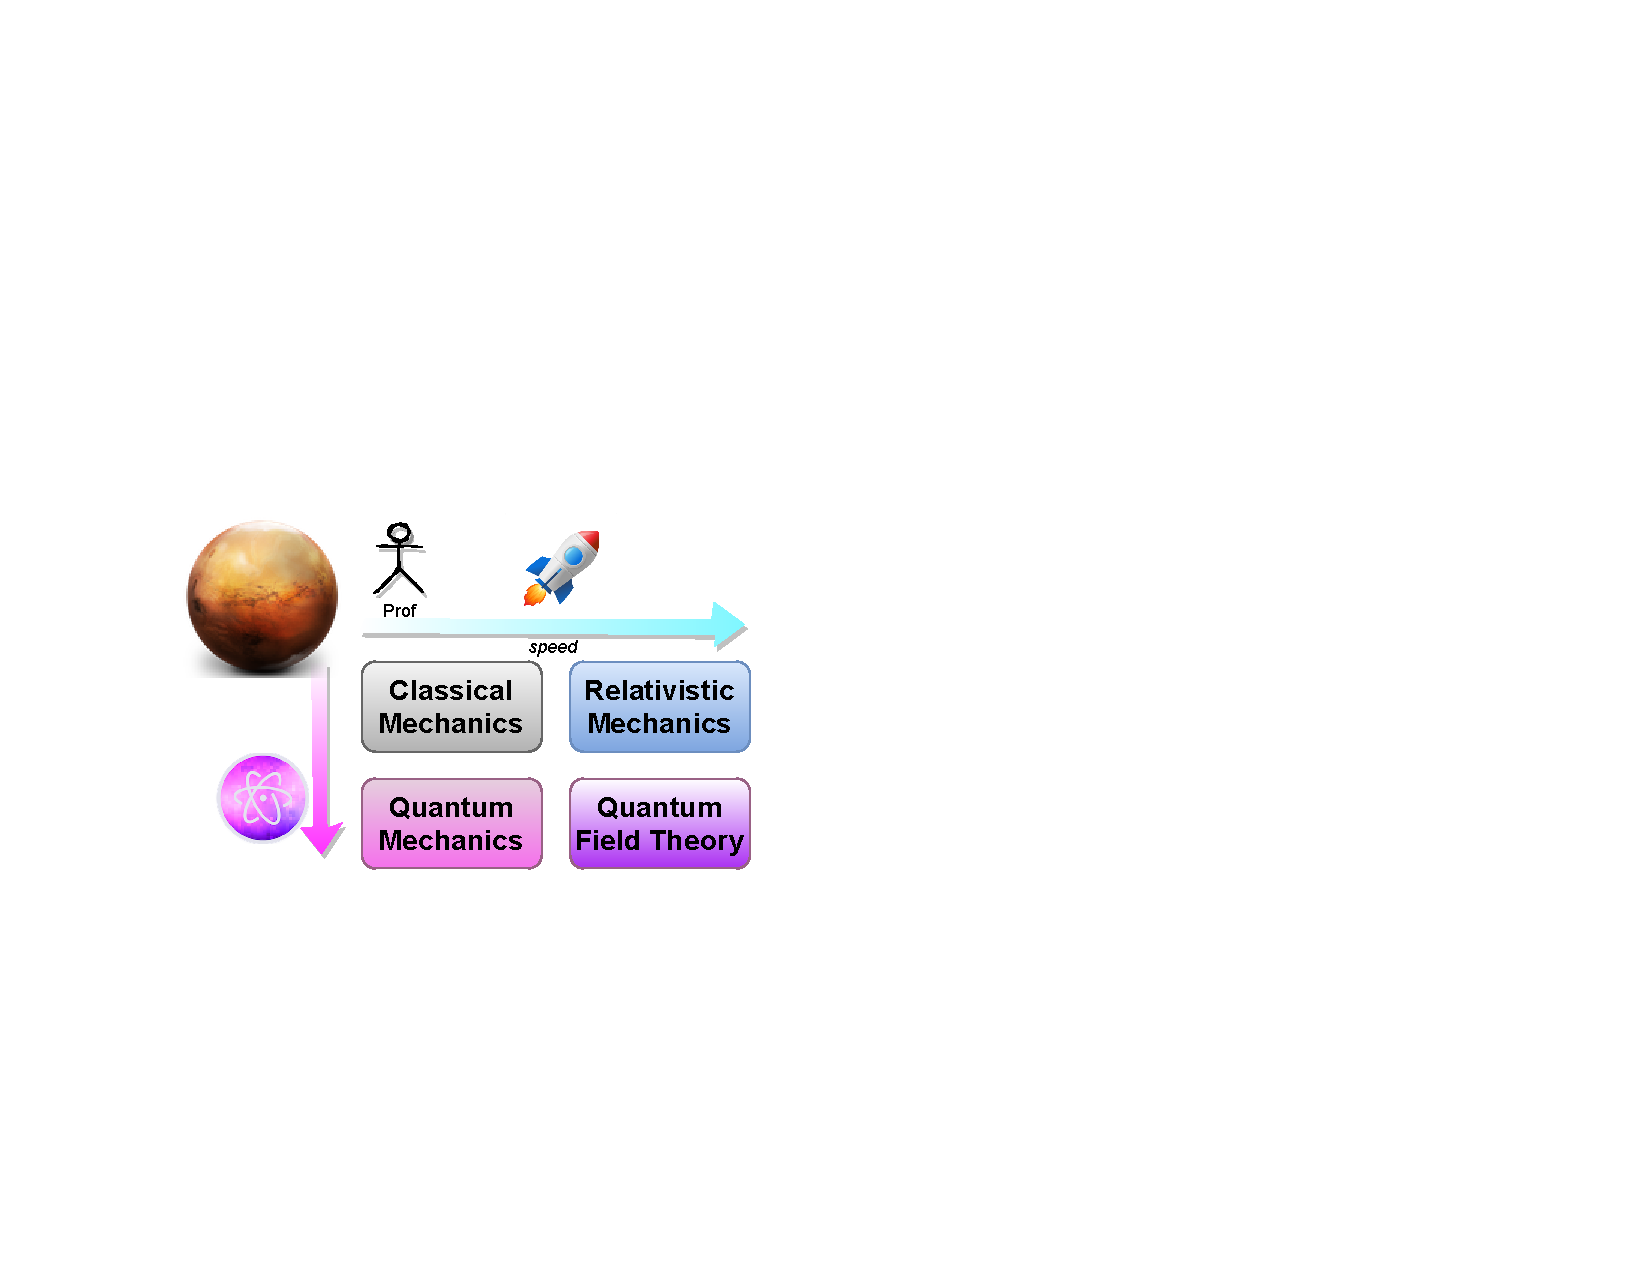
\includegraphics[width=\columnwidth]{stat-mech-overview.pdf}
\caption{EM waves in a black box with sides of length $L$}
\end{figure}


\begin{enumerate}
\item Basics of probability
\item mean, median, var, std, ...
\end{enumerate}


\clearpage
\section{Binary State Systems: April 2}

\clearpage
\section{Equilibrium: April 7}

\subsection{Review of Last Week}
\begin{itemize}
\item \textbf{Fundamental Assumption of Statistical Mechanics:} "An isolated system in uqilibrium is equally likely to be found in any of the microstates available to it."

\item $g =$ "the multiplicity"; the number of accessible micro states for a given set of extensive parameters (e.g. U, N, V)

\item If all such states are equally likely, then \textit{the probability distribution is uniform}: $P_i = 1/g$

\item The mean value or "Expectation value" of an observable $\mathcal{A}$ is defined 
  $\Braket{\mathcal{A}} = \displaystyle \sum_{i} \mathcal{A}_i P(i)$

\item Fluctuations are \textit{\textbf{tiny}}: For N >> 1, quantities like $\Delta U/U$ go as $1/\sqrt{N}$

\item This is a consequence of the Central Limit Theorem. Ensembles of many varying distributions sum up to a Gaussian distribution.

\end{itemize}

\subsubsection{Collection of N magnetic spins}
\begin{equation}
g(N,s) = \frac{N!}{(N/2 + s)! (N/2-s)!}
\end{equation}
Using Stirling's Approximation (cf. \href{http://mathworld.wolfram.com/StirlingsApproximation.html}{MathWorld}):
\begin{equation}
log(N!) = N log(N) - N + \frac{1}{2}log(2 \pi N)
\end{equation}
\begin{figure}[h]
\centering
\includegraphics[width=\columnwidth]{Figures/Stirling.pdf}
\caption{Comparison of various approximations to N!}
\end{figure}
after some substitutions, we find that

\begin{equation}
g(N,s) = 2^N \sqrt{\frac{2}{\pi N}} exp\bigg[-\frac{1}{2}\bigg(\frac{s}{\sigma_s}\bigg)^2\bigg]
\end{equation}
where $\sigma_s = \sqrt{N}/2$ is the standard deviation of the Gaussian probability 
distribution of $s$, the spin excess.

\subsection{Thermal Equilibrium for Two Systems}
Let us consider two non-interacting systems. Each system is a box with a collections of
spins. Box 1 has $N_1$ total atoms and an initial spin excess of $s_1$.
The combined multiplicity of these 
two systems (before we allow them to interact) is (using the same logic that we used to consider
our binary model of coin flips) just the product of the individual multiplicities:
\begin{align}
g_{tot} &= g_1 \times g_2 \\
        &= \frac{2}{\pi} \frac{1}{\sqrt{N_1 N_2}} 2^{N_1 + N_2} exp\bigg[-2\bigg(\frac{s_1^2}{N_1} + 
        \frac{s_2^2}{N_2}\bigg)\bigg]
\label{eq:ginit}
\end{align}
Rather than consider some artificial magnetic spin exchange interaction, let us instead
turn on an external magnetic field, such that the energy of each system becomes
$U_i = -2 m B s_i$, where $m$ is the magnetic moment of each atom and $B$ is the magnetic
field. We then bring the boxes into contact, such that it is possible to interchange energy
between the two system. The total spin and the total energy will remain conserved
(e.g. $U = U_1 + U_2$). For this two system example, we do not let the number of atoms in
each box change: $N_1 = const, N_2 = const$.

After the energy exchange begins, the two systems move from their 
initial state (Eq.~\ref{eq:ginit}) into a new state
\begin{equation}
g_{tot} = g_1(U_1^\prime) \times g_2(U_2^\prime)
\end{equation}
with more accessible microstates.

We would like to find what the new equilibrium state is. In other words, 
what is the most probable state after the two (sub)systems have been in contact 
long enough to come into equilibrium?
\begin{figure}[h]
\centering
\includegraphics[width=\columnwidth]{Figures/TwoSystemMultiplicity.pdf}
\caption{The multiplicity functions for two systems before (Blue and Red) and after (Purple) being put 
	into thermal contact.}
\end{figure}

To find this, we would like to find the stationary point for the combined multiplicity function. To do this we set the $dg/dU = 0$:

\begin{equation}
dg = \bigg(\frac{\partial g_1}{\partial U_1}\bigg)_{N_1} g_2~dU_1 +
     \bigg(\frac{\partial g_2}{\partial U_2}\bigg)_{N_2} g_1~dU_2 = 0  
\label{eq:maxg}
\end{equation}

Since energy is conserved, any energy gained by one sub-system is equal
to the amount lost by the other: $dU_1 = -dU_2$. Dividing through by
$g_1 g_2$, we find the condition for \textit{thermal equilibrium}:

\begin{equation}
\bigg(\frac{\partial log(g_1)}{\partial U_1}\bigg)_{N_1} = 
\bigg(\frac{\partial log(g_2)}{\partial U_2}\bigg)_{N_2}
\label{eq:maxmicro}
\end{equation}



\clearpage
\section{Entropy: April 9}

\subsection{Entropy}
\label{s:Entropy}
The number of microstates is a huge number! Its much easier to work with the
logarithm of such large numbers. The logarithm is also convenient since adding
systems together requires just adding their logarithms, rather than multiplying
the number of microstates.

So we define \textit{\textbf{entropy}} as:
\begin{equation}
\sigma \equiv log(g)
\end{equation}
This is a dimensionless (unitless) quantity (its just the logarithm 
of a large number...). \\

As we saw in the previous lecture, the combined system moves from its initial configuration
(where system 1 and 2 have the energies $U_1$ and $U_2$, respectively) into the one which
is \emph{overwhelmingly} likely. Recall that our conclusion from the discussion of thermal
equilibrium is that for macroscopic systems (e.g. with $N \gtrsim 10^{15}$...actually the
transition from micro to macro is a fuzzy concept, but this is an OK estimate for now), the
chances of the energy being even 1\,ppm different from the most probable value are astronomically unlikely (really? Yes - see the Shakespeare, monkeys, and typewriters
problem in this week's problem set).

\begin{equation}
\bigg(\frac{\partial \sigma_1}{\partial U_1}\bigg)_{N_1} = 
\bigg(\frac{\partial \sigma_2}{\partial U_2}\bigg)_{N_2}
\label{eq:Teq}
\end{equation}

This tendency of the system to always move into a configuration which maximizes
the number of accessible micro-states ($g$) is a just another way of stating the
2$^{\rm nd}$ Law of Thermodynamics: The entropy of a closed system will always 
increase until the system reaches equilibrium.

\epigraph{Turning and turning in the widening gyre \\
The falcon cannot hear the falconer; \\
Things fall apart; the centre cannot hold; \\
Mere anarchy is loosed upon the world,...}{\textit{William B. Yeats, 1919}}

\subsection{Temperature}
\label{s:Temperature}

Intuitively, we know that putting things in contact brings them to the same temperature
(cf. the "Brain Freeze" available at the Red Door Cafe). So we want this to be
implied by Eq.~\ref{eq:Teq}.

From Eq.~\ref{eq:Teq}, we could pick $\tau, 1/\tau, or -\tau,...$, but we want temperature
to correspond to our human definitions of it. Zero temperature should be very low energy
and temperature should rise as we put more kinetic energy into the particles, so we define
it like so:
\begin{equation}
\frac{1}{\tau} \equiv \bigg(\frac{\partial \sigma}{\partial U}\bigg)_{N}
\label{eq:Temp}
\end{equation}

\subsection{The Laws of Thermodynamics}

\subsubsection{The 0$^{\rm th}$ Law: Thermometers}
\href{http://en.wikipedia.org/wiki/Zeroth_law_of_thermodynamics}{Wikipedia:Zeroth Law}

From our definitions of temperature and thermal equilibrium 
(cf. \cref{eq:Temp,eq:Teq}), 
we see that if $\tau_1 = \tau_3$ and $\tau_2 = \tau_3$, then 
$\tau_1 = \tau_2$. 
In this example, $\tau_3$ is the temperature of the thermometer we are 
using to establish the equivalence of the temperatures of our two example 
systems (1 and 2). Why is this seemingly trivial statement worthy
of being a so-called "Law of Thermodynamics"? 



\subsubsection{The 1$^{\rm st}$ Law: No Free Lunch}
\begin{figure}[h]
\centering
\includegraphics[width=0.5\columnwidth]{Figures/Carnot_heat_engine_2.pdf}
\caption{Schematic diagram of Carnot's Heat Engine \\
	\url{http://commons.wikimedia.org/wiki/File:Carnot_heat_engine_2.svg}}
\end{figure}
A concise statement of the 1$^{\rm st}$ Law is:
\begin{equation}
\Delta U = Q + W
\label{eq:FirstLaw}
\end{equation}
where $\Delta U$ is the total internal energy of our system, $W$ is the
mechanical work done \emph{to the system}\footnote{note the sign convention
here; the work is done to the system and not by the system}, and $Q$ is
the \textit{heat}. But what is heat? We all know what it is intuitively,
but it is important to define it such that it can be used consistently in
our studies of statistical mechanics. As defined in Ch.~8 of the textbook,
heat is the energy transfer between two systems which are in thermal contact.
It does not include work or any transfer of material. In the Carnot example
above, $W = Q_H - Q_C$. Systems where $W > Q_H - Q_C$ are called
perpetual motion machines of the first kind, and are known to be
impossible to conservation of energy.

\subsubsection{The 2$^{\rm nd}$ Law: Everything Runs Down}
As we saw above in Sec.~\ref{s:Entropy}, when a system begins in a
non-equilibrium state (such as the one where we first bring the two
sub-systems into contact), it always moves in the direction which
increases the entropy:\footnote{This is put to music in the song "Unsustainable", from the rock band Muse's album "The 2nd Law". Some Gaussian distributions and combinatorics are displayed for affect in their music video:
\href{https://www.youtube.com/watch?v=EF_xdvn52As}{YouTube:Unsustainable}} pieces of a broken wine glass "never" reassemble
into a whole glass. When we run the film backwards, we see this happen,
but it seems that there is a preferred to direction to the 
flow of time. This is often referred to as the 
Arrow of TIme~\footnote{\href{http://www.wired.com/2014/04/quantum-theory-flow-time/}{2004 Wired article} on how quantum correlations may be the underlying basis for the arrow of time}

For the heat engine example above, $\Delta \sigma = Q_C/\tau_C - Q_H/\tau_H$.
In order for $\Delta \sigma$ to be positive, we must have $\tau_H > \tau_C$,
since $Q_H \ge Q_C$.



\epigraph{The law that entropy always increases, holds, I think, the supreme position among the laws of Nature. If someone points out to you that your pet theory of the universe is in disagreement with Maxwell's equations --- then so much the worse for Maxwell's equations. If it is found to be contradicted by observation --- well, these experimentalists do bungle things sometimes. But if your theory is found to be against the second law of thermodynamics I can give you no hope; there is nothing for it but to collapse in deepest humiliation.}
{\textit{Sir Arthur S. Eddington, 1928}}

\subsubsection{The 3$^{\rm rd}$ Law: Nernst Theorem}





\clearpage
\section{Boltzmann Factor: April 14}


\subsection{The Boltzmann Factor}
An important problem in Statistical Physics, is to find the probability
of finding a system in a state $s$ of energy $\epsilon_s$. We already
know how to do this for closed systems, but most systems are, in reality, open systems -- that is, they are in contact with a large thermal bath or reservoir. This might be the rest of the room (in the case of a tiny experiment) or the rest of the city (in the case that the system is a building) or even the rest of the universe (in astrophysical or cosmological cases). \\

So lets take our little system $\mathcal{S}$ and put in contact with our large reservoir $\mathcal{R}$ with initial energy $U_0$ and temperature $\tau_R$. Now we put our system in thermal (and later, mechanical) contact with the reservoir such that the new energy of the reservoir is $U_0 - \epsilon_s$. Now 
$\mathcal{R}$ can be in any of its $g_R(U_0 - \epsilon_s)$ microstates, just as we saw in last week's \textit{microcanonical} picture. \\

For a given state $s$, there is no degeneracy; the multiplicity, $g_s = 1$. So the probability of finding the total system ($\mathcal{S} + \mathcal{R}$) in the state where $\mathcal{S}$ has energy $\epsilon_s$, is just dependent on the multiplicity $g_R$: $P(s) \propto g_R(U_0 - \epsilon_s)$. Since 
$U_0 \gg \epsilon_s$, we can use the Taylor expansion to find a simplified form:

\begin{equation}
\log g_R = \sigma_R(U_0 - \epsilon_s) \simeq 
	\sigma_R(U_0) - 
	\epsilon_s \bigg(\frac{\partial \sigma_R}{\partial U_R}\bigg) +
	\mathcal{O}(\epsilon_s^2)
\end{equation}

Since $(\partial \sigma_R/\partial U_R) = 1/\tau_R$, we can rewrite the proportionality for the probability as:

\begin{equation}
P(s) \propto exp(-\epsilon_s/\tau_R)
\end{equation}

This is \textbf{one the most practically useful results in statistical physics}: it allows us to compute the relative probability of the system being in different energy states. This expression, $exp(-\epsilon_s/\tau_R)$, is called the
\emph{Boltzmann Factor}.


\subsection{Partition Function}
We would like to normalize the probability so that 
$\sum_s P(s) = 1$. To do this, we just sum over all possible energy states.

\begin{equation}
P(s) = \frac{exp(-\epsilon_s/\tau_R)}{\sum_s exp(-\epsilon_s/\tau_R} = 1
\end{equation}
and where we will define the \emph{Partition Function}\footnote{an oddly named function for sure} as
\begin{equation}
Z(\tau_R) \equiv \sum_s exp(-\epsilon_s/\tau_R
\end{equation}

\subsection{Pressure}

\subsection{Free Energy}


\textbf{Summary}

\begin{itemize}
\item The probability of finding a system (in microstate $s$ with
	energy $\epsilon_s$, in thermal equilibrium with a reservoir 
	at temperature $\tau_R$) is proportional to the 
	\emph{Boltzmann factor} $P(s) \propto exp(-\epsilon_s/\tau_R)$.

\item To normalize $P(s)$ properly ($\sum_{s} P(s) = 1$), we divide
	the Boltzmann factor by the sum over all energy states.
	$P(s) = exp(-\epsilon_s/\tau_R)/Z$, where 
	$Z(\tau_R) \equiv \sum_{s} exp(-\epsilon_s/\tau_R)$. $Z$ is called the
	partition function.

\item For a compressible system, if we change the volume slowly and by
	a small amount, the entropy won't change (\textit{isentropic}). This
	is defined as \textit{pressure}: $p = -(\partial U/\partial V)_\sigma$

\item The picture of closed system with an accessible number of microstates
	and associated entropy is the \emph{microcanonical ensemble}. In this picture, the energy, volume, and number of the system is fixed.

\item The \emph{canonical ensemble} is the similar picture, but with 
	the system now in thermal equilibrium with a heat bath. Consequently,
	the temperature is now fixed, but the energy of the system is not.

\end{itemize}






\clearpage
\section{Helmholtz Free Energy and the Ideal Gas: April 16}

\clearpage
\section{Ideal Gas I: April 16}
\label{s:IdealGasI}
As a first look at the Ideal Gas model, we start by assuming that we have $N$ identical point like particles in a box. These particles do not interact with each other and, by the virtue of being point-like, we can ignore the rotational and vibrational energies which real molecules have.\\

We can then procede to solve for the quantum wavefunctions and energies just as we do for the standard "particle-in-a-box" problem (cf. K\&K, Ch.\,1, pp.\,9-10).
\begin{equation}
\hat{H} \Braket{\Psi} = E \Braket{\Psi}
\end{equation}

\begin{figure}[h]
\centering
\includegraphics[width=0.7\columnwidth]{Figures/ParticleBoxPlot.pdf}
\caption{Example wavefunction for a particle in a square 2D box 
	with sides of length $L$}
\end{figure}

For this potential (the box), the Hamiltonian is just that for a free 
particle:

\begin{equation}
\hat{H} = -\frac{\hbar^2}{2 m} \nabla^2
\end{equation}

This type of wave equation has solutions of the form $A \sin{x} + B \cos{x}$.
By including the boundary conditions that $\Braket{\Psi} = 0$ when
($x, y, z$) = $0$ or $L$, we can eliminate the cosine terms and we are left
with:
\begin{equation}
\Psi(x,y,z) = \mathcal{C} \sin(n_x \frac{\pi}{L} x) \sin(n_y \frac{\pi}{L} y) \sin(n_z \frac{\pi}{L} z)
\end{equation}
where $\mathcal{C}$ is the normalization constant. After normalization (to set the total probability equal to 1), we can get the quantized energies by plugging into the Schr\"odinger Equation above:
\begin{equation}
\epsilon_n = \frac{\hbar^2}{2 m}\bigg(\frac{\pi}{L} \bigg)^2 (n_x^2 + n_y^2 + n_z^2)
\label{eq:IdealGasEnergies}
\end{equation}

\subsection{Partition Function}
We can now begin using our standard canonical ensemble 'toolbox' to derive relationships for the macroscopic observables of the system. The Boltzmann factor for a single particle is just $exp(-\epsilon_n/\tau)$ and the Partition function is
\begin{equation}
Z_1 = \sum_{n_x} \sum_{n_y} \sum_{n_z} e^{-\epsilon_n/\tau}
\end{equation}
Unsurprisingly, we would like to convert this summation into an integral in order to solve it, but is this really valid? It is, but only if the error between the sum and the series is small; i.e. true if $\epsilon_{n+1} - \epsilon_n \ll \tau$. 
At room temperature, $\tau = k_B T = (1.38 \times 10^{-23} J/K)(300 K)$. 
To convert to eV, we divide by the electron charge ($1.602 \times 10^{-19} C$), 
so $\tau \simeq \frac{1}{40} eV$. The
prefactor in \cref{eq:IdealGasEnergies} is $\sim 10^{-16} eV$ for a $1~mm^3$ box,
so the approximation made by using an integral instead of an infinite series is extremely accurate even at the nano-Kelvin temperature now achievable through modern cryogenic methods.\\

We can then perform the integral by noting that its separable into three integrals (one for each $n_i$) and that each integral is of the form $\int exp(-\alpha^2 x^2)$, which we have done before and can look up in Appendix A of K\&K or 
\href{http://www.wolframalpha.com/input/?i=integrate\%20exp(-a\%5E2\%20x\%5E2)\%20from\%20x\%3D0..infinity}{Wolfram Alpha}.
\begin{align}
Z_1 &= L^3 \bigg(\frac{2 \pi \hbar^2}{m \tau}\bigg)^{-3/2} \\
    &= n_Q V
\end{align}
where $V = L^3$ and 
\begin{equation}
n_Q \equiv \bigg(\frac{2 \pi \hbar^2}{m \tau}\bigg)^{-3/2}
\label{eq:QuantConc}
\end{equation} 
which we define as the \emph{Quantum Concentration}. Since 
for most gases at
room temperature, the single particle density ($1/V$) is much smaller than
$n_Q$, $Z_1 \ll 1$, and the \textit{classical approximation} is valid. Otherwise, we would have to consider the quantum entanglement between the molecules.\\

For distinguishable particles, the multi-particle partition function is just the product of the individual particle partition functions, just as the multi particle multiplicity is the product of the single particle multiplicities. Since the
gas particles are identical, we weight it by the number of identical permutations:
\begin{equation}
Z_N = \frac{Z_1}{N!} = \frac{(n_Q V)^N}{N!}
\label{eq:IdealGasZ}
\end{equation}



\subsection{The Ideal Gas Law}
To understand the macroscopic properties of the N particle ideal gas, we can start with our expression for the Free Energy in terms of the Partition Function:
\begin{align}
F &= -\tau~\log Z_N \\
  &= -\tau~(N \log Z_1 - \log N!) \\
  &= -\tau~(N \log{n_Q V} - \log N!)
\end{align}

From \cref{eq:dFdX}, we have that
\begin{align}
p &= -\bigg(\frac{\partial F}{\partial V}\bigg)_\tau \\
  &= N \tau / V
\end{align}
and changing from our 'fundamental' units to SI units, we recover the Ideal Gas Law:
\begin{equation}
\boxed{p V = N k_B T}
\end{equation}





















\clearpage
\section{Planck Black Body: April 21}

Let's consider now a system which is similar to the previous two (Ideal Gas and small System in a large Reservoir), but with a significant twist. Instead of a system where the constituents have a mass, we want to study what happens inside of a 
black\,\footnote{Here, by 'black', I mean that the walls of the box are a 'perfectly' absorbing conductor. This is a little counterintuitive; you know that very good conductors (e.g. aluminum, copper, silver) are very reflective and \emph{not} perfectly absorbing. Nevertheless, this turns out to be a valid approximation for what we are looking into and, in fact, works well with boxes of almost any generic properties.} box in thermal equilibrium with a Reservoir. Instead of particles of a gas, we will be working with \textit{photons}, the massless quanta of electromagnetic radiation. In the end we would like to end up with all the now usual concepts: total energy, entropy, pressure (yes, even light has a 
pressure~\footnote{cf. solar sails}), and the energy distribution (i.e. can 
we predict what color something will be?). \\

\begin{figure}[h]
\centering
\includegraphics[width=0.3\columnwidth]{Figures/245px-photon_waves.png}
\caption{EM waves in a black box with sides of length $L$}
\end{figure}


We'll start off with the assumption\,\footnote{which will be qualified later} that the energy of each photon of angular frequency $\omega$($=2 \pi \nu$) will just be proportional to the frequency:
\begin{equation}
\epsilon = \hbar \omega
\end{equation}
To an extremely good approximation, photons do not interact with each other (i.e. you cannot deflect a laser beam with another laser beam). So there can, in principle, be many photons with the same energy inside the box. We'll denote the occupancy of each mode as $s$, and so the energy per mode will be $\epsilon_s = s \hbar \omega$. The total energy will then just be an appropriately weighted sum over all the available modes.\\

At a temperature $\tau$, the Boltzmann factor for a \textit{single} mode 
is $e^{-s \hbar \omega / \tau}$. So the partition function for that mode is:
\begin{align}
Z &= \sum_{s=0}^{\infty} e^{-s \hbar \omega / \tau} \\
  &= \frac{1}{1 - e^{-\hbar \omega / \tau}}
\label{eq:PartPlanck}
\end{align}
where we have used the relation $\sum_{s=0}^{\infty} x^s = 1/(1-x)$, 
valid when $x < 1$. \\

\subsection{The Planck Distribution}
At this point we can utilize all of the tools we have developed during the study of the canonical ensemble in Chapter 3. We know that the probability 
distribution can just be computed from the Boltzmann factor and the partition 
function (cf.\,\cref{eq:PofS}):
\begin{equation}
P(s) = e^{-s \hbar \omega / \tau} \bigg[ 1 - e^{-\hbar \omega / \tau} \bigg]
\end{equation}
and to find the average occupancy of each mode we just multiply by $s$ and sum over all states:
\begin{align}
\Braket{s} &= \sum_{s=0}^{\infty} s~P(s) \\
           &= \frac{1}{Z} \sum_{s=0}^{\infty} s~e^{-s \hbar \omega / \tau}
\end{align}
We can perform the sum here by transforming it into a more familiar form. To do this note that:
\begin{equation}
\sum s~e^{-s x} = -\frac{d}{dx} \sum e^{-s x}
\end{equation}
and the right hand side can be summed in the same way as \cref{eq:PartPlanck}, above.
So finally we arrive at the expression for the average occupancy:
\begin{equation}
\boxed{\Braket{s} = \frac{1}{e^{\hbar \omega / \tau} - 1}}
\end{equation}
which is the \emph{Planck distribution} for the occupancy of a single mode in thermal equilibrium with a heat bath of temperature $\tau$. The average energy in each mode is:
\begin{equation}
\boxed{\Braket{\epsilon} = \Braket{s} \hbar \omega= 
\frac{\hbar \omega}{e^{\hbar \omega / \tau} - 1}}
\end{equation}
Its interesting to look at the high and low temperature (or equivalently, the low and high frequency) limits of this expression. \\

At high temperatures, where 
$\tau \gg \hbar \omega$, we can expand the denominator ($e^x \simeq 1 + x$) and see
that $\Braket{\epsilon} \to \tau$. This is the 'classical limit'; the energy is just
proportional to the temperature and there is no evidence of quantization.\\

At low temperatures, where $\tau \ll \hbar \omega$, the denominator becomes large
and $\Braket{\epsilon} \to 0$. So a black box will tend towards zero energy in the
electromangetic field~\footnote{neglecting the ground state energy of 
$\frac{1}{2}\hbar \omega$ per mode} as well as zero occupancy. \\

This highlights another interesting difference between
a box of ideal gas molecules and a box of radiation: \emph{the photon number is
not a conserved quantity}. As we will see soon, the same is true for 
\textit{phonons}, the acoustic excitations in a solid.


\subsection{The Stefan-Boltzmann Law}
We would like to now move on to the main goal, which is to find the total energy,
entropy, etc. for the blackbody, summing over all the modes.

\begin{equation}
U = 2 \sum_n \Braket{\epsilon_n} = 
\sum_n \frac{\hbar \omega_n}{exp(\hbar \omega_n / \tau) - 1}
\end{equation}
where we have followed the convention from K \& K pp. 92-93 which describes
the accounting for the modes allowed in the box (similar reasoning as we use
for waves on a string and particle in a box). The factor of 2 comes from accounting
for the 2 polarizations of the radiation field and $\omega_n = n \pi c/L$.\\

We can replace the sum over the indices ($n_x, n_y, n_z$) with a triple integral
to make the computation easier. This is valid as long as the box is not small
with respect to the wavelength of the relavent radiation field ($L \gg c/\omega$).\\

To make the integral easier, we'll convert it from Cartesian coordinates to
spherical coordinates and replace the volume element $dn_x dn_y dn_z$, with
the spherical volume element $4 \pi\,n^2 dn$.
\begin{align}
U &= 2 \times \frac{1}{8} \times 4 \pi 
\int_{0}^{\infty} n^2 \frac{\hbar \omega_n}{exp(\hbar \omega_n / \tau) - 1} dn \\
  &= \frac{L^3 \tau^4}{\pi^2 \hbar^3 c^3} \int_{0}^{\infty} \frac{x^3}{e^x - 1} dx \\
  &= \frac{\pi^2 L^3 \tau^4}{15 \hbar^3 c^3}
\label{eq:BBenergy}
\end{align}
where the factor of 2 is for both polarizations, the $1/8$ because we only want to consider one octant of the spherical volume (where the wavenumbers are positive), and the $4 \pi$ covers the angular part of the volume integral. We then have made the substitution $x = \pi \hbar c n / L \tau$ to get the dimensionless 
integral. We can look up~\footnote{you can do it for yourself in a few steps if you want: multiply top and bottom by $e^{-x}$ and then recall our infinite sum for 
$1/(1-x)$} the integral in a book or Mathematica to find that its $\pi^4/15$.

Its useful to also look at the spectral distribution of the energy. To get that
we can rewrite the integrand above as:
\begin{align}
\frac{U}{V} &= \int_{0}^{\infty} u_{\omega} d\omega \\
	        &= \frac{\hbar}{\pi^2 c^3} \frac{\omega^3}{e^{\hbar \omega/\tau} - 1}
\end{align}
where we've moved the volume ($V = L^3$) over to the left hand side and used
our expression from above to replace $n$ with $\omega$. This
\textit{spectral density}, $u_{\omega}$, is called the
\emph{Planck Black Body Spectrum} and the theoretical and experimental work which
gave rise to it was the first evidence for $\hbar$ and was the birth of
Quantum Mechanics.

\begin{figure}[ht]
\centering
\includegraphics[width=0.7\columnwidth]{Figures/BlackbodySpectrum_loglog_150dpi_en.png}
\caption{Blackbody Radiation Intensity Spectral density. \\
	From \url{https://commons.wikimedia.org/wiki/File:BlackbodySpectrum_loglog_150dpi_en.png}}
\end{figure}



\clearpage
\section{Ideal Gas: April 16}
Introduction to the Ideal Gas model.

%%%%%%%%%%%%%%%%%%%%%%%%%%%%%%%%%%%%%%%%%%%%%%%
\end{document}
